\documentclass{beamer}
\usepackage{graphicx}
\usepackage{tikz}
\usetikzlibrary{shapes,arrows}
\usepackage{tikz}
%\usecolortheme{seahorse}
  \setbeamertemplate{footline}[page number]
\usepackage{multirow}
\setbeamertemplate{navigation symbols}{}
\setbeamertemplate{frametitle}[default][center]
\setbeamerfont{frametitle}{shape=\scshape}
\usepackage{color}

\usepackage{csquotes}

\usepackage{xcolor}

\usepackage[flushleft]{threeparttable}

{\title{\textsc{Econ 352 - Income Disparity Among Countries and Endogenous Growth} \\ \tiny (See Williamson Ch. 8)}
\author{Trevor S. Gallen}
\date{}
\begin{document}
\renewcommand*{\inserttotalframenumber}{\pageref{lastframe}}


\setbeamertemplate{caption}{\raggedright\insertcaption\par}

\begin{frame}
\titlepage
\end{frame}

\begin{frame}
\frametitle[alignment=center]{Introduction}
\begin{itemize}
\item We saw our simple Solow Growth model
\bigskip
\item And talked about what does and doesn't cause growth
\bigskip
\item And how to measure $z$
\bigskip
\item Does it have anything to say about why some countries are rich and some countries are poor?
\end{itemize}
\end{frame}

\begin{frame}
\frametitle[alignment=center]{Convergence}
\begin{itemize}
\item Let's revisit our old model:
$$K'=\frac{szf(k)}{1+n}+\frac{(1-\delta)K}{1+n}$$
\item Note that $K^*$, the steady state, is the same for two countries, no matter their $K_0$!
\bigskip
\item Prediction:  all countries should ``converge" to the same level of capital
\end{itemize}
\end{frame}

\begin{frame}
\frametitle[alignment=center]{The Steady State is Identical, no matter $K_0$}
\begin{figure}
\centering
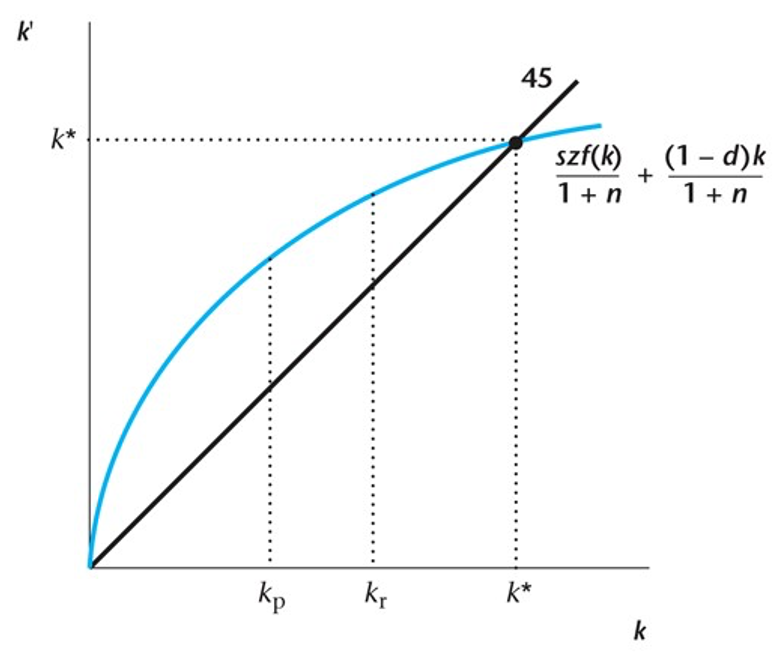
\includegraphics[scale=0.5]{Figures/W_Fig_8pt1.png}
\end{figure}
\end{frame}

\begin{frame}
\frametitle[alignment=center]{Convergence in Income Per Worker}
\begin{figure}
\centering
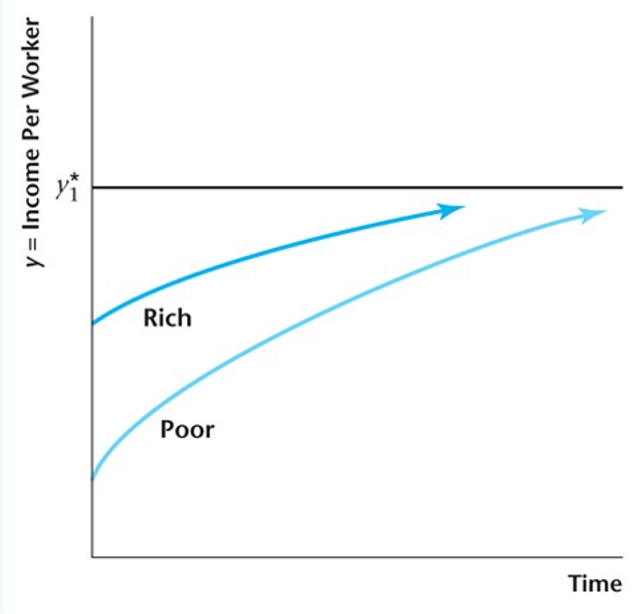
\includegraphics[scale=0.5]{Figures/W_Fig_8pt2.png}
\end{figure}
Poor countries should ``catch up" to rich ones
\end{frame}

\begin{frame}
\frametitle[alignment=center]{Convergence in Aggregate Income }
\begin{figure}
\centering
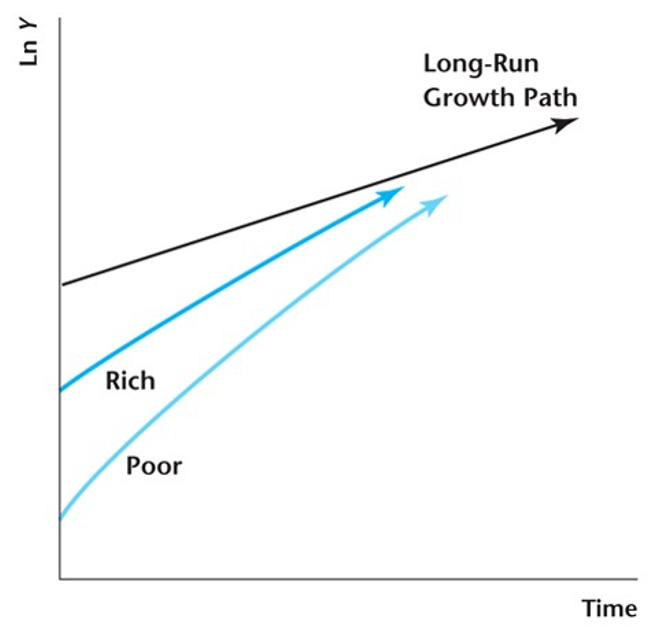
\includegraphics[scale=0.5]{Figures/W_Fig_8pt3.png}
\end{figure}
Poor countries should ``catch up" to rich ones, even with shared TFP growth in $z$
\end{frame}

\begin{frame}
\frametitle[alignment=center]{Concrete Prediction(?)}
\begin{itemize}
\item Poor countries should ``catch up" to rich ones
\bigskip
\item Important assumption is that all parameters $z$, $s$, $n$ $\delta$ are the same!
\bigskip
\item What if technology isn't spread evenly?  $z$ differences, for instance
\bigskip
\item Why would $z$ differ?
\bigskip
\begin{itemize}
\item ``Learning by doing"
\item Barries to technology adoption
\item Country-specific efficiency (taxes/regulation, for instance)
\end{itemize}
\item These can cause a failure to converge
\end{itemize}
\end{frame}

\begin{frame}
\frametitle[alignment=center]{Convergence in Aggregate Income }
\begin{figure}
\centering
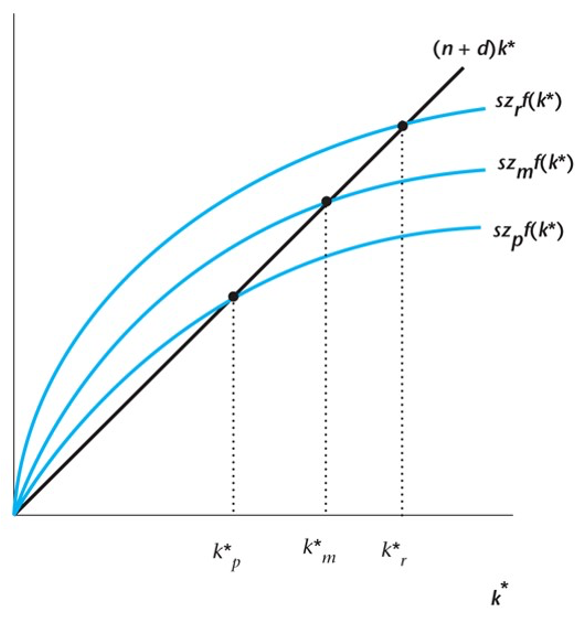
\includegraphics[scale=0.5]{Figures/W_Fig_8pt4.png}
\end{figure}
Failure to converge
\end{frame}



\begin{frame}
\frametitle[alignment=center]{Endogenous Growth}
\begin{itemize}
\item The great success of the Solow Growth model is to tell us what is \emph{not} causing growth (labor hours and capital).
\bigskip
\item But its big failure is that it doesn't tell us what \emph{does}, only productivity ``z," which is taken as exogenous
\bigskip
\item Endogenous growth models try to explain changes in $z$ over time
\bigskip
\item We'll work through a ``Lucas 1988" endogenous growth model
\bigskip
\item Basic idea:  a representative consumer splits time between work and learning (think ``research")
\end{itemize}
\end{frame}


\begin{frame}
\frametitle[alignment=center]{Lucas Endogenous Growth Model: Representative Consumer}
\begin{itemize}
\item Our worker now has $H^s$ units of human capital
\bigskip
\item The choose a fraction of time to work $u$, and their ``efficiency units of labor" are $uH^s$.  Someone with $H^s=2$ would produce twice as much as someone with $H^s=1$, if they both worked the same amount.
\bigskip
\item Total earnings are $wuH^s$, which equal consumption:
$$C=wuH^s$$
\item Human capital increases as a function of time spent ``researching" $1-u$:
$$(H^s)'=b(1-u)H^s$$
\item Where $b$ is the ``efficiency" of research 
\end{itemize}
\end{frame}

\begin{frame}
\frametitle[alignment=center]{Lucas Endogenous Growth Model: Representative Firm}
\begin{itemize}
\item Production is:
$$Y=zuH^d$$
\item So that profit is:
$$\pi=Y-wuH^d$$
\item Plugging in,
$$\pi=zuH^d-wuH^d=(z-w)uH^d$$
\item Taking FOC's wrt $H^d$:
$$\frac{\partial \pi }{\partial H^d}=0\Rightarrow (z-w)=0\Rightarrow w=z$$
\item Wages are a measure of human capital: $wH^d=zH^d$
\end{itemize}
\end{frame}

\begin{frame}
\frametitle[alignment=center]{Lucas Endogenous Growth Model: Competitive Equilibrium}
\begin{itemize}
\item From the budget constraint:
$$C=zuH$$
\item Human capital:
$$H'=b(1-u)H$$
\item Rephrasing for human capital growth:
$$\frac{H'}{H}-1=b(1-u)-1$$
\item The growth rate of human capital increases if $b$ increases or $u$ decreases
\bigskip
\item More efficient educational system will have higher growth rate of human capital: no convergence
\bigskip
\item And for $C$:
$$\frac{C'}{C}-1=\frac{zuH'}{zuH}-1=\frac{H'}{H}-1=b(1-u)-1$$
\end{itemize}
\end{frame}

\begin{frame}
\frametitle[alignment=center]{Equilibrium Wage Rate (supply \& demand) }
\begin{figure}
\centering
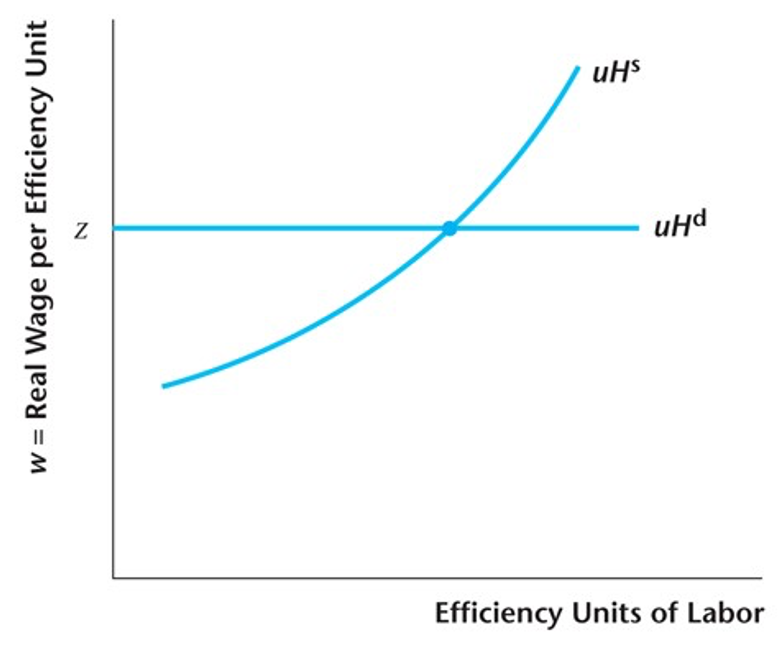
\includegraphics[scale=0.5]{Figures/W_Fig_8pt5.png}
\end{figure}
\end{frame}

\begin{frame}
\frametitle[alignment=center]{Human capital accumulation }
\begin{figure}
\centering
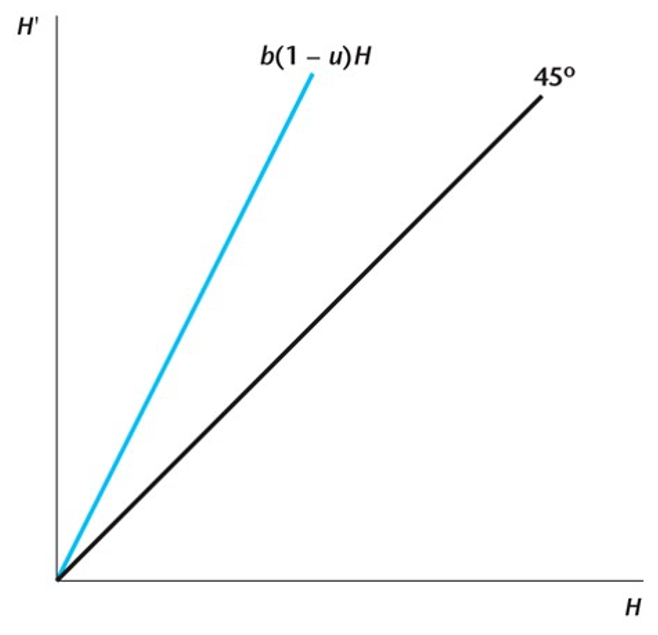
\includegraphics[scale=0.5]{Figures/W_Fig_8pt6.png}
\end{figure}
Growth is unbounded!
\end{frame}



\begin{frame}
\frametitle[alignment=center]{Lucas Endogenous Growth Model: Policy}
\begin{itemize}
\item We now have a model of \emph{endogenous} growth!
\bigskip
\item Government policy can affect growth rates
\bigskip
\item If the government increases efficiency of human capital accumulation $b$, then we would expect more growth!
\bigskip
\item What happens to $C$ tomorrow if we decreased $u$ today (studied more, worked less)?
\end{itemize}
\end{frame}

\begin{frame}
\frametitle[alignment=center]{Lucas Endogenous Growth Model: Policy}
\begin{itemize}
\item Consumption today:  
$$C=zuH$$
\item Consumption growth:
$$\frac{C'}{C}=b(1-u)-1$$
\item When $u$ decreases,\emph{growth} picks up but $C$ falls initially!
\end{itemize}
\end{frame}

\begin{frame}
\frametitle[alignment=center]{Effect of a decrease in $u$ on consumption path}
\begin{figure}
\centering
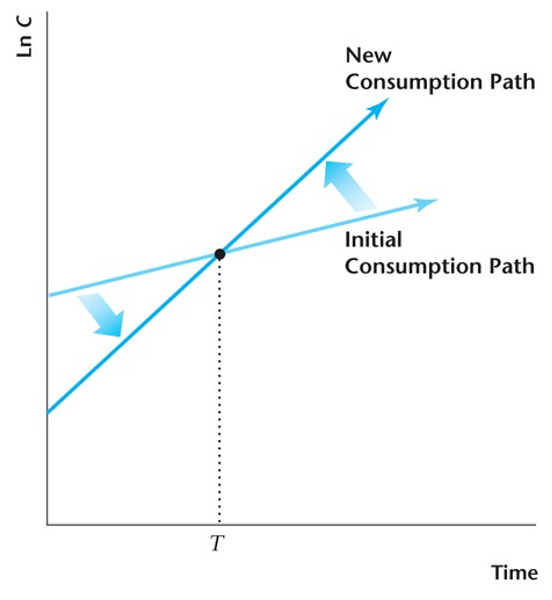
\includegraphics[scale=0.5]{Figures/W_Fig_8pt7.png}
\end{figure}
Tradeoff between today and tomorrow
\end{frame}


\begin{frame}
\frametitle[alignment=center]{Endogenous growth and convergence}
\begin{itemize}
\item One big takeaway is that in this model, we do not have convergence/``catch-up" growth causing a convergence between countries
\bigskip
\item ``Catch up" on $z$ may help, but there can still be divergence
\bigskip
\item How do we reconcile the fact that rich countries seem to have converged but poor countries have not?
\bigskip
\item One is if $b$ and $u$ are similar among rich countries, and human capital accumulation in one country ``splils over" to another
\bigskip
\item Similarly, if the high human capital in poorer countries earn more in rich countries, there may be a ``brain drain" reducing the wages of all remaining workers, helping divergence
\end{itemize}
\end{frame}


\begin{frame}
\frametitle[alignment=center]{Endogenous Growth Can Remove Convergence}
\begin{figure}
\centering
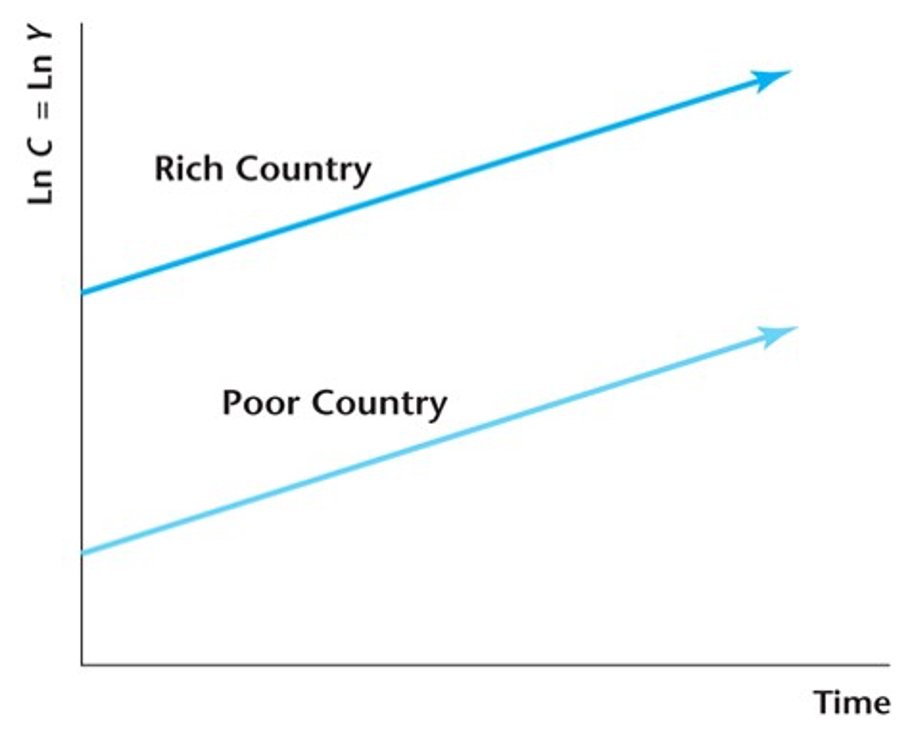
\includegraphics[scale=0.5]{Figures/W_Fig_8pt8.png}
\end{figure}
\end{frame}








\end{document}